\documentclass[11pt]{article}

\usepackage{authblk}
\usepackage[a4paper,margin=2cm]{geometry}
\usepackage[utf8]{inputenc}
\usepackage{mathptmx} % times roman, including math
\usepackage[hyphens]{url}
\usepackage{doi}
\usepackage{hyperref}
\usepackage[numbers,sort]{natbib}
\usepackage{amsmath}
\usepackage{amssymb}
\usepackage{amsthm}
\usepackage{stmaryrd} % \llbracket etc.
\usepackage{algorithm}
\usepackage{algpseudocode} % layout for algorithmicx package, provides "algorithmic" environment for pseudocode
\usepackage{setspace}
\usepackage{csquotes}
\usepackage{tikz}
\usetikzlibrary{arrows.meta}
\hyphenation{da-ta-cen-ter da-ta-cen-ters time-stamp time-stamps time-stamped Grish-chen-ko}
\frenchspacing

\newtheorem{proposition}{Proposition}

\begin{document}
\sloppy
\title{OpSets: Concurrent Datatypes with Sequential Specifications}
%\title{OpSets: Sequential Specifications for Concurrent Editing}
\author[1]{Martin Kleppmann\thanks{Corresponding author. Email: martin.kleppmann@cl.cam.ac.uk}}
\author[1]{Victor B.\ F.\ Gomes}
\author[2]{Dominic P.\ Mulligan}
\author[1]{Alastair R.\ Beresford}
\date{}

\affil[1]{Department of Computer Science and Technology, University of Cambridge, UK}
\affil[2]{Security Research Group, Arm Research, Cambridge, UK}

\maketitle

\begin{center}
Regular Paper
\end{center}

\begin{abstract}
This paper introduces OpSets, a new framework for specifying and reasoning about the semantics of replicated datatypes that provide eventual consistency in a distributed system.
First, we show our approach is simpler than previous work by using OpSets to succinctly specify a variety of abstract data types, including maps, sets, lists, text, graphs, trees, and registers.
Our data types are also composable, enabling the construction of complex data structures such as a list of maps.
We then demonstrate the utility of OpSets as a tool to support the analysis of existing algorithms for eventual consistency.
In particular, we highlight an important new correctness property in collaborative text editing.
This property has traditionally been overlooked and can result in awkward interleaving of text, and we use OpSets to specify the required correctness property and prove that one existing algorithm supports this property while other published algorithms do not. 
Finally, we also show how OpSets can be used to make improvements in the state-of-the-art, by providing a simple specification of an atomic move operation for complex abstract datatypes, something which had previously been thought impossible without locking.
We use the Isabelle/HOL proof assistant throughout to formalise the OpSets approach and produce mechanised proofs of correctness of the main claims in this paper, thereby eliminating the ambiguity of previous informal approaches and ruling out reasoning errors that could occur in handwritten proofs.
\end{abstract}
\clearpage

\section{Introduction}

A common requirement across a great variety of systems is that several participants may concurrently access and manipulate some shared data structure, such as a text document, a spreadsheet, or a database.
In doing so, it is important that the shared data satisfies certain \emph{consistency guarantees}.
For example, strong consistency models such as serializability \cite{Kleppmann:2017wj} or linearizability \cite{Herlihy:1990jq} attempt to make a system behave like a single sequentially executing node, even when it is in fact replicated and concurrent.
An unavoidable downside of these models is that they require waiting for synchronous network communication before any operation or transaction is allowed to complete \cite{Davidson:1985hv,Gilbert:2002il}.
Thus, in a system with strong consistency, a node cannot make progress while it is offline or partitioned from other nodes.

On the other hand, \emph{eventual consistency} \cite{Bailis:2013jc,Burckhardt:2014hy,Terry:1994fp,Vogels:2009ca} allows each participant to modify a local copy (\emph{replica}) of a shared data structure while offline, but its definition is very weak: \emph{``if no new updates are made to the shared state, all nodes will eventually have the same data.''}
The premise \emph{if no new updates are made} may never be true, for example if the shared state is continually modified because the system is never quiescent.
Moreover, the final state that is eventually reached is unconstrained: nothing in the definition of eventual consistency specifies which states are legal.

Conflict-free Replicated Data Types, or CRDTs \cite{Shapiro:2011wy,Shapiro:2011un}, are abstractions for replicated state that have received significant attention in recent years (see Section~\ref{sec:relwork}).
The primary correctness property for CRDTs is \emph{convergence} \cite{Shapiro:2011un,Gomes:2017gy}, defined as: \emph{``whenever any two replicas have applied the same set of updates, they are in the same state''} (even if each replica applies the updates in a different order).
Convergence is a stronger property than eventual consistency, but it also fails to define what the converged state should be.

In this work we introduce \emph{Operation Sets} (or \emph{OpSets} for short), a novel approach for specifying the semantics of replicated datatypes, and reasoning about algorithms for concurrent data access and manipulation.
We go beyond merely ensuring replica convergence: the OpSets approach is a form of executable specification that precisely defines the permitted states of a replica after some set of updates has been applied.

Our contributions in this paper are as follows:

\begin{itemize}
\item In Section~\ref{sec:approach} we introduce the OpSet, a new abstraction for specifying and reasoning about the consistency properties of concurrently editable data structures.
On top of this abstraction, we specify a variety of abstract datatypes (maps, sets, lists, text, graphs, trees, and registers) in Sections~\ref{sec:datatypes} and~\ref{sec:tree}, and we argue that our specification is both simpler and more precise than previous efforts to specify the semantics of these data structures.

\item In Section~\ref{sec:bad-merge} we highlight an important correctness property for collaborative text editing that has been overlooked by prior work in this area.
Our specification is, to our knowledge, the first that correctly captures this property.
We then review a selection of text editing CRDTs from the literature, prove that one satisfies our specification, and identify several others that fail to satisfy our correctness property.

\item In Section~\ref{sec:tree} we demonstrate, for the first time, how an atomic move operation can be defined for a tree CRDT.
This operation can be used to move a subtree to a new position within the tree, or to rename a key in a map, or to reorder items in a list.
The OpSets approach enables a simple definition of this operation that had previously been thought to be impossible without locking \cite{Najafzadeh:2017vk}.

\item Using the Isabelle/HOL proof assistant~\cite{DBLP:conf/tphol/WenzelPN08} we formalise the OpSets approach, producing mechanised proofs of correctness of the main claims in this paper.
In particular, we prove that our list specification is strictly stronger than the recent specification of collaborative text editing by Attiya et al. \cite{Attiya:2016kh}, and we prove that our tree specification satisfies the required invariants.
By using mechanised proofs we eliminate the ambiguity of previous informal approaches, and rule out reasoning errors that could occur in handwritten proofs.
\end{itemize}

\section{The OpSets Approach}\label{sec:approach}

At a high level, consistency models for distributed data systems can be classified into two categories:
\begin{description}
\item[Strong consistency models] such as serialisability or linearisability \cite{Herlihy:1990jq} attempt to make a system behave like a single sequentially executing node, even when it is in fact replicated and concurrent.
An unavoidable downside of these models is that they require waiting for synchronous network communication before any operation or transaction is allowed to complete \cite{Davidson:1985hv,Gilbert:2002il}.
Thus, a node cannot make progress while it is offline or partitioned from other nodes.
In a formal sense, enforcing a strong consistency model is equivalent to consensus \cite{Chandra:1996cp,Herlihy:1991gk}, which implies that the algorithm cannot be guaranteed to terminate in an asynchronous system \cite{Fischer:1985tt}.

\item[Weak consistency models] are employed by systems that prioritise availability over strong consistency; for example, systems that require nodes to be able to make progress while offline or while partitioned from other nodes.
In such systems, each node typically reads and manipulates a local copy of the shared state, and propagates any changes to that state asynchronously to other nodes.
Examples of weak consistency models in this category are \emph{causal consistency} \cite{Attiya:2015dm,Mahajan:2011wz,Lloyd:2011hz} and \emph{eventual consistency} \cite{Bailis:2013jc,Burckhardt:2014hy,Terry:1994fp,Vogels:2009ca}.
\end{description}

In this work we focus on the latter category of weak consistency models.
However, as we shall demonstrate shortly, the OpSets approach allows us to specify our consistency model more precisely than existing techiques permit.

\subsection{Eventual Consistency is Insufficient}\label{sec:eventual-consistency}

Eventual consistency is usually informally defined as follows: \emph{if no new updates are made to the shared state, all nodes will eventually have the same data}.
This is a very weak definition for several reasons:
\begin{itemize}
\item The premise, \emph{if no new updates are made}, may never be true (if the shared state is continually modified because the system is never quiescent).
In that case, eventual consistency becomes a vacuous statement.

\item Many trivial algorithms satisfy the requirement of converging towards the same state.
For example, a system could simply discard writes, and thus converge to a state in which operations have been ignored.
Although such a system would not be useful in practice, the definition of eventual consistency does not capture the requirement that writes should be persistent.

\item In a system that allows nodes to make progress while they are partitioned from other nodes, it is inevitable that the local state of individual nodes might diverge due to concurrent modifications.
Such divergent states must then be merged at a later time, when communication between the nodes is restored.
Even if we require that this merge operation does not discard data that has been written, eventual consistency does not specify which states should be considered valid results of the merge operation.
\end{itemize}

\subsection{Introducing OpSets}\label{sec:opsets-intro}

The OpSets approach is a simple abstraction that allows us to be more precise about the consistency properties of a replicated data system.
We assume that the system consists of a set of \emph{nodes} connected by a network.
These nodes concurrently access some \emph{shared data structure}, which may be a relational database (consisting of rows in tables), a text document (an ordered list of characters), a vector-graphics document (a tree of records describing graphical objects), or any other kind of data structure.

We assume that each node has a local copy of the shared data structure, which it can read and modify without locking or any other coordination with other nodes.
Whenever a node makes a modification to that structure, it records the change as an \emph{operation}.
For example, an operation may describe a particular insertion at a particular position in a document.
We assume that each operation has a unique identifier that is different from any other operation generated anywhere in the system.
For example, the identifier may consist of a unique node identifier and a sequence number.

Each node locally maintains a set of operations, the \emph{OpSet}.
Whenever a node makes a change, it adds the corresponding operation to its OpSet, and also broadcasts the operation to other nodes.
Whenever a node receives an operation from another node, that operation is also added to the recipient's local OpSet.
Any operations that are lost in the network are retransmitted as necessary.
Operations remain immutable throughout this process.

Thus, the OpSet is a monotonically growing set of operations, and every operation is eventually contained in the OpSet of every node from which it is not permanently partitioned.
(To deal with unbounded growth, we discuss garbage collection later in this paper.)
Any two communicating nodes can merge their OpSets using the standard set union, which is commutative, associative, and idempotent, ensuring that communicating nodes converge towards the same OpSet contents.

\subsection{Data Structures as Queries}\label{sec:queries}

Existing algorithms for maintaining replicated state, such as CRDTs, describe how a node's local state may be manipulated as a result of operations.
We now depart from this convention and present an alternative formulation of replicated data structures.

In the OpSets approach, we require that the shared data structure is never manipulated directly.
Instead, we assume the existence of a pure function that takes an OpSet as input, and returns the current state of the shared data structure according to the OpSet.
The transformation from OpSet to data structure is deterministic and depends only on the contents of the OpSet -- regardless of whether that data structure is a relational database, a text document, a tree, a graph, or anything else.
All nodes in the system employ the same transformation function.
Consequently, whenever any two nodes have the same OpSet, their view of the shared data structure must also be equal.

One can regard the OpSet of being a \emph{database of facts}, containing all of the changes ever made to the shared data.
The function that deterministically transforms this database into some derived data structure is a \emph{query}.
The resulting data structure is, in database terminology, a \emph{materialized view} onto the underlying set of operations.

We show in the following sections how many practical data structures can be expressed as queries.
For now we note that this construction trivially ensures eventual consistency: as two nodes converge towards the same OpSet contents, any data structure that is deterministically derived from the OpSet must also converge.
By using a deterministic query language to derive the data structure from the OpSet, we can~-- by construction~-- rule out any violations of this convergence property.

Moreover, we can take advantage of a rich body of existing research on query languages and materialized view maintenance.
When a new operation is added to the OpSet, a query execution engine can determine the change to the derived data structure that results from the addition of the new operation.
Determining this change to the query result is known as \emph{incremental view maintenance}, and we build upon extensive prior research in this area.

\subsection{Operation Serializability}\label{sec:op-serial}

Like in the definition of eventual consistency in Section~\ref{sec:eventual-consistency}, deriving a data structure from an OpSet ensures convergence, but it does not define how an operation should take effect.
To refine our correctness properties, we must define the expected semantics of operations.

Normally, reasoning about the semantics of concurrently modified data structures is difficult and error-prone.
However, the OpSets model enables us to reason about operation semantics in a sequential way, and directly extend the sequential semantics to arbitrary concurrent executions.

We previously required that every operation has a unique identifier.
We now assume that we also have a total ordering on operation identifiers, and that this total order is a linear extension of the partial order that captures their causal dependencies (the \emph{happens-before} relation).
That is, whenever a node generates a new operation, the identifier of the new operation must be greater than that of any existing operation in the OpSet of the node generating the new operation.
This requirement can easily be met by using Lamport timestamps \cite{Lamport:1978jq} as identifiers.

Now observe that for any OpSet there exists a unique sequence of operations, containing all operations of the OpSet in ascending order of their identifier.
We can specify the semantics of each operation~-- that is, the effect of the operation on the query result~-- when applied in this sequential order.
Since we know that the query result is determined entirely by the OpSet, we know that even if the operations arrive at a node in any arbitrary order, the final query result must be the same as if they had been applied sequentially in order of ascending identifier.

In other words, we have \emph{operation serializability}: the data structure derived from an OpSet is equal to the outcome of applying the operations in their serial order.
It is therefore sufficient for us to define the semantics of each operation under serial execution, and we know that this definition will also define its semantics in arbitrary concurrent executions: any state in a concurrent execution corresponds to some OpSet, and the operations in that OpSet are serializable.

\section{Specifying a Graph of Lists, Maps, and Registers}\label{sec:datatypes}

We now make the OpSets approach concrete by defining example semantics for commonly-used data structures: maps (which associate values with user-specified keys) and lists (linear sequences of values).
The map datatype can also represent a set (by using keys as members of the set, and ignoring values).
The list datatype can also represent text (by mapping each character to a list element).
In both lists and maps the values may be primitives (such as numbers or strings), or references to other map or list objects.
Using these references we can construct arbitrary object graphs, including cycles of object references, like in object-oriented programming languages.
In \S~\ref{sec:tree} we will show how to restrict this object graph so that it conforms to a tree structure.

We treat each key of a map, and each element of a list, as a multi-value register.
That is, if there are several concurrent assignments to the same map key or list element, our datatype preserves all concurrently written values.
Thus, reading a map key or list element may return multiple values, which may be merged explicitly by the user.
Assigning a new value to a map key or list element overwrites all causally preceding values.
Different register behaviour, such as last-writer-wins (arbitrarily picking one of the concurrently written values as winner), can easily be defined, as we show later.

\subsection{Generating Operations}\label{sec:datatypes-gen}

An OpSet for these datatypes may contain six types of operation:
\begin{itemize}
    \item $(\mathit{id},\, \mathsf{MakeMap})$ creates a new, empty map object that is identified by $\mathit{id}$.
    \item $(\mathit{id},\, \mathsf{MakeList})$ creates a new, empty list object that is identified by $\mathit{id}$.
    \item $(\mathit{id},\, \mathsf{MakeVal}(\mathit{val}))$ associates the ID $\mathit{id}$ with the primitive value $\mathit{val}$ (e.g.\ a number, string, or boolean).
        This operation is used to ``wrap'' any primitive value, allowing $\mathsf{Assign}$ operations (see below) to always use IDs as values, regardless of whether the value is a primitive value, or a reference to a map or list object.
    \item $(\mathit{id},\, \mathsf{InsertAfter}(\mathit{ref}))$ creates a new list element with ID $\mathit{id}$, and inserts it into a list.
        If $\mathit{ref}$ is the ID of a prior $\mathsf{MakeList}$ operation, then the new element is inserted at the head of that list.
        Otherwise $\mathit{ref}$ must be the ID of an existing list element (i.e.\ a prior $\mathsf{InsertAfter}$ operation), in which case the new list element is inserted immediately after the referenced list element.
        Note that the $\mathsf{InsertAfter}$ operation does not associate a value with the new list element; that is done by a subsequent $\mathsf{Assign}$ operation.
    \item $(\mathit{id},\, \mathsf{Assign}(\mathit{obj}, \mathit{key}, \mathit{val}, \mathit{prev}))$ assigns a new value to a key within a map (if $\mathit{obj}$ is the ID of a prior $\mathsf{MakeMap}$ operation), or to a list element (if $\mathit{obj}$ is the ID of a prior $\mathsf{MakeList}$ operation).
        In the case of map assignment, $\mathit{key}$ is the user-specified key to be updated, which may be any primitive value such as a string or integer.
        In the case of a list, $\mathit{key}$ is the ID of the list element to be updated (i.e.\ the ID of a prior $\mathsf{InsertAfter}$ operation).
        $\mathit{val}$ is the ID of the value being assigned, which may identify a $\mathsf{MakeMap}$, $\mathsf{MakeList}$, or $\mathsf{MakeVal}$ operation.
        $\mathit{prev}$ is the set of IDs of prior $\mathsf{Assign}$ operations to the same key in the same object, which are overwritten by the present operation.
    \item $(\mathit{id},\, \mathsf{Remove}(\mathit{obj}, \mathit{key}, \mathit{prev}))$ removes a key-value pair from a map, or an element from a list.
        As with $\mathsf{Assign}$, $\mathit{obj}$ is the ID of the prior $\mathsf{MakeMap}$ or $\mathsf{MakeList}$ operation that created the object being updated, and $\mathit{key}$ identifies the key or list element being removed.
        $\mathit{prev}$ is the set of IDs of prior $\mathsf{Assign}$ operations to the same key in the same object, which are removed by the present operation.
\end{itemize}

\ifarxiv
  \noindent
  Pseudocode for generating these operations is given in Appendix~\ref{sect:appendix:generating-ops}.
\else
  \noindent
  Pseudocode for generating these operations is provided in an appendix of the extended version of this paper.
\fi


\subsection{Interpreting Operations}\label{sec:datatypes-interp}

We use the sequential OpSet interpretation given in \S~\ref{sec:op-serial}.
To encode the current state of map and list data structures we use a pair of relations $(E,\, L)$:

\begin{description}
    \item[The element relation $E \subseteq (\mathrm{ID} \times \mathrm{ID} \times (\mathrm{ID} \cup \mathrm{Key}) \times \mathrm{ID})$]
        is a set of 4-tuples containing the values currently assigned to map keys and list elements.
        If $(\mathit{id}, \mathit{obj}, \mathit{key}, \mathit{val}) \in E$, then an $\mathsf{Assign}$ operation with ID $\mathit{id}$ updated the object with ID $\mathit{obj}$, assigning the value with ID $\mathit{val}$ to the map key or list element $\mathit{key}$.
        If $\mathit{obj}$ references a list object, $\mathit{key}$ is the ID of an element in the list relation $L$ (see below).
        If $\mathit{obj}$ references a map object, any primitive value such as string or integer may be used as $\mathit{key}$.
    \item[The list relation $L \subseteq (\mathrm{ID} \times \mathrm{ID})$] is a set of pairs that indicates the order of list elements.
        If $(\mathit{prev}, \mathit{next}) \in L$, that means the list element with ID $\mathit{prev}$ is immediately followed by the list element with ID $\mathit{next}$.
        We use $(\mathit{last}, \bot) \in L$ to indicate that list element $\mathit{last}$ has no successor.
        To indicate that $\mathit{head}$ is the first element in the list $\mathit{obj}$ (i.e.\ $\mathit{obj}$ is the ID of the $\mathsf{MakeList}$ operation that created the list) we have $(\mathit{obj}, \mathit{head}) \in L$.
\end{description}

\noindent
Initially, both relations are empty; that is, we have $\llbracket\emptyset\rrbracket = \mathit{InitialState} = (\emptyset,\, \emptyset)$.
We can then define the interpretation of the six operation types as follows:
\begin{align*}
    \mathit{interp}\big[(E,\, L),\; &(\mathit{id},\, \mathsf{Assign}(\mathit{obj}, \mathit{key}, \mathit{val}, \mathit{prev})) \big] \;=\\
    &\Big( \big\{ (\mathit{id}', \mathit{obj}', \mathit{key}', \mathit{val}') \in E \mid
    \mathit{id}' \notin \mathit{prev} \big\} \;\cup\;
    \big\{ (\mathit{id}, \mathit{obj}, \mathit{key}, \mathit{val}) \big\},\; L \Big) \\[5pt]
    %%%%%%%%%%
    \mathit{interp}\big[(E,\, L),\; &(\mathit{id},\, \mathsf{Remove}(\mathit{obj}, \mathit{key}, \mathit{prev})) \big] \;=\\
    &\Big( \big\{ (\mathit{id}', \mathit{obj}', \mathit{key}', \mathit{val}') \in E \mid
    \mathit{id}' \notin \mathit{prev} \big\},\; L \Big) \\[5pt]
    %%%%%%%%%%
    \mathit{interp}\big[(E,\, L),\; &(\mathit{id},\, \mathsf{InsertAfter}(\mathit{ref})) \big] \;=\\
    &\left\{
        \arraycolsep=0pt \def\arraystretch{1.2}
        \begin{array}{ll}
            (E,\, L) & \text{if } \nexists\,n.\; (\mathit{ref},\, n) \in L\\[3pt]
            \Big(E,\; \big\{ (p,n) &\;\in L \mid p \neq \mathit{ref} \big\} \;\cup\;
            \big\{ (\mathit{ref}, \mathit{id}) \big\} \;\cup\;
            \big\{ (\mathit{id}, n) \mid (\mathit{ref}, n) \in L \big\} \Big)\\
            & \text{if } \exists\,n.\; (\mathit{ref},\,n) \in L
        \end{array} \right. \\[5pt]
    %%%%%%%%%%
    \mathit{interp}\big[(E,\, L),\; &(\mathit{id},\, \mathsf{MakeList}) \big] \hspace{21.1pt}=\;
    \Big( E,\; L \;\cup\; \big\{(\mathit{id},\, \bot)\big\}\Big) \\[1pt]
    %%%%%%%%%%
    \mathit{interp}\big[(E,\, L),\; &(\mathit{id},\, \mathsf{MakeMap}) \big] \hspace{17.6pt}=\; (E,\; L) \\[5pt]
    \mathit{interp}\big[(E,\, L),\; &(\mathit{id},\, \mathsf{MakeVal}(\mathit{val})) \big] \;=\; (E,\; L)
\end{align*}

The interpretation of $\mathsf{Assign}$ and $\mathsf{Remove}$ updates only $E$ and leaves $L$ unchanged; conversely, the interpretation of $\mathsf{InsertAfter}$ and $\mathsf{MakeList}$ updates only $L$.
Both the $\mathsf{Assign}$ and $\mathsf{Remove}$ interpretations remove any tuples from causally prior assignments (those whose IDs appear in $\mathit{prev}$), but leave any tuples from concurrent assignments unchanged.
This is the behaviour of a multi-value register; if a last-writer-wins register is required, the condition $\mathit{id}' \notin \mathit{prev}$ can be changed to $\mathit{obj}' \neq \mathit{obj} \;\vee\; \mathit{key}' \neq \mathit{key}$, which removes any existing tuples with the same object ID and key.

The interpretation of $\mathsf{InsertAfter}$ resembles the insertion into a linked list, as illustrated in Figure~\ref{fig:list-insert}.
For example, to interpret $(\mathit{id},\, \mathsf{InsertAfter}(\mathit{ref}))$, if we have $(\mathit{ref}, \mathit{next}) \in L$, we remove the pair $(\mathit{ref}, \mathit{next})$ from L, and add the pairs $(\mathit{ref}, \mathit{id})$ and $(\mathit{id}, \mathit{next})$ to $L$.
Thus, the new list element $\mathit{id}$ is inserted between $\mathit{ref}$ and $\mathit{next}$.

\begin{figure}
\centering
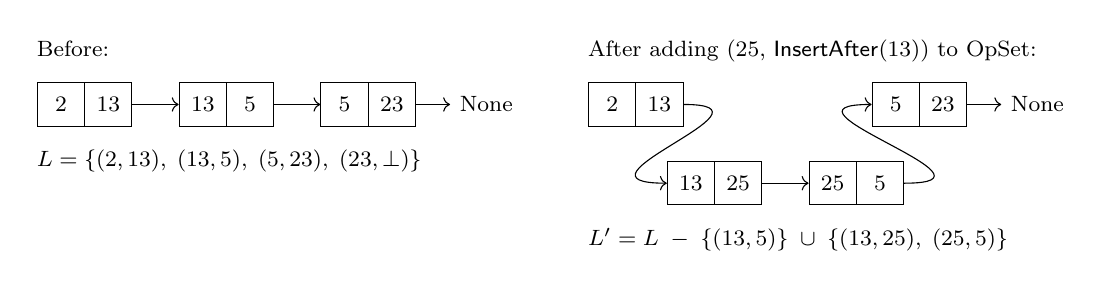
\begin{tikzpicture}
  \tikzstyle{every node}=[anchor=base,minimum width=6mm,text height=7pt,text depth=2pt,font=\footnotesize]
  \node [anchor=west] at (-7,1.7) {Before:};
  \node [anchor=west] at (-7,0.3) {$L = \{ (2, 13),\; (13, 5),\; (5, 23),\; (23, \bot) \}$};
  \node [anchor=west] at (0,1.7) {After adding $(25,\, \mathsf{InsertAfter}(13))$ to OpSet:};
  \node [anchor=west] at (0,-0.7) {$L' = L \;-\; \{(13, 5)\} \;\cup\; \{(13, 25),\; (25, 5)\}$};
    \matrix [column sep={6mm,between origins},nodes=draw,matrix anchor=west] at (-7,1) {
    \node (l1a) {2};  & \node (l1b) {13}; &&
    \node (l2a) {13}; & \node (l2b) {5};  &&
    \node (l3a) {5};  & \node (l3b) {23}; &&
    \node (l4a) [draw=none] {None}; \\
  };
  \draw [->] (l1b) -- (l2a);
  \draw [->] (l2b) -- (l3a);
  \draw [->] (l3b) -- (l4a);
  \matrix [column sep={6mm,between origins},nodes=draw,matrix anchor=west] at (1,0) {
    \node (n1) {13}; & \node (n2) {25}; &&
    \node (n3) {25}; & \node (n4) {5}; \\
  };
  \matrix [column sep={6mm,between origins},nodes=draw,matrix anchor=west] at (0,1) {
    \node (r1a) {2};  & \node (r1b) {13}; &&&&&
    \node (r3a) {5};  & \node (r3b) {23}; &&
    \node (r4a) [draw=none] {None}; \\
  };
  \draw [->] (r1b.east) .. controls (2.7,1) and (-0.3,0) .. (n1.west);
  \draw [->] (n2) -- (n3);
  \draw [->] (n4.east) .. controls (5.6,0) and (2.3,1) .. (r3a.west);
  \draw [->] (r3b) -- (r4a);
\end{tikzpicture}
\caption{Illustration of the interpretation of an $\mathsf{InsertAfter}$ operation.}\label{fig:list-insert}
\end{figure}

Note that $L$ never shrinks, it only ever grows through interpreting $\mathsf{InsertAfter}$ operations.
When a list element is removed by a $\mathsf{Remove}$ operation, the effect is that all values are removed from the list element in the element relation $E$, but the list element remains in $L$ as a \emph{tombstone}, so that any concurrent $\mathsf{InsertAfter}$ operations can still locate the referenced list position.
Thus, from a user's point of view a list element only exists if it has at least one associated value in the $E$ relation; any list elements without an associated value should be ignored.

\section{Discussion: Merging Text Edits}\label{sec:bad-merge}

The datatypes we have specified can support a wide range of applications.
For example, the list datatype can be used to implement a collaborative text editor: by treating the text as a list of individual characters, every edit can be expressed as a sequence of insertion or deletion operations on the list.

The problem of collaborative text editing has been studied extensively, using two main approaches: Operational Transformation and CRDTs.
We discuss this prior work in Section~\ref{sec:relwork}.
We will now highlight a scenario that, to our knowledge, has not been considered by any previous work on collaborative text editing.

Consider the execution illustrated in Figure~\ref{fig:bad-merge}.
In this example, two users are concurrently editing a text document that initially reads ``Hello!''.
The user on the left changes it to read ``Hello Alice!'', while concurrently the user on the right changes the document to read ``Hello Charlie!''.
When the concurrent edits are merged, the algorithm randomly interleaves the two insertions of ``~Alice'' and ``~Charlie'' character by character, resulting in an unreadable jumble of characters.

\begin{figure}
\centering
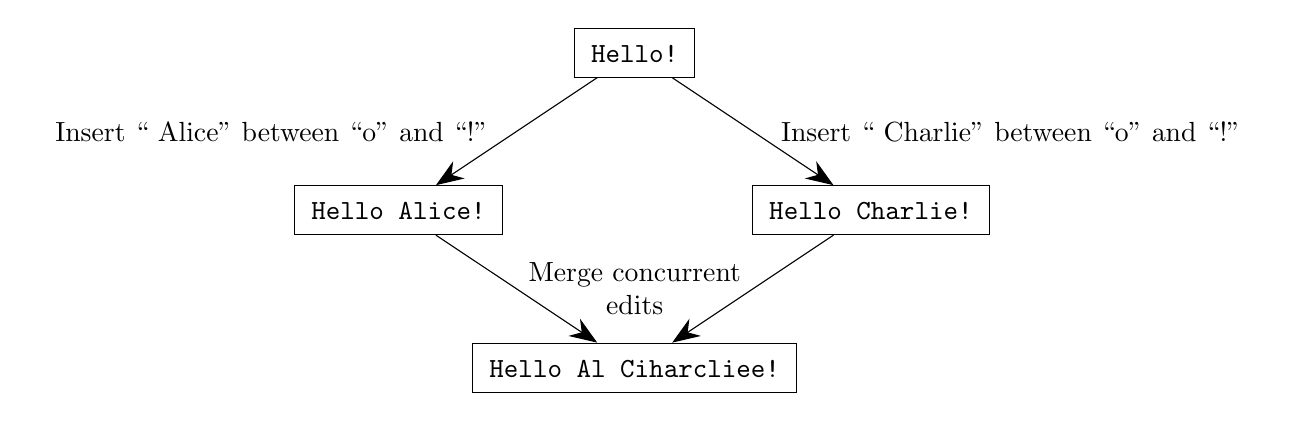
\begin{tikzpicture}
  \tikzstyle{box}=[rectangle,draw,inner xsep=6pt,text height=9pt,text depth=2pt]
  \tikzstyle{every path}=[draw,-{Stealth[length=3.5mm]}]
  \node [box] (start) at (3,4) {\texttt{Hello!}};
  \node [box] (left)  at (0,2) {\texttt{Hello Alice!}};
  \node [box] (right) at (6,2) {\texttt{Hello Charlie!}};
  \node [box] (merge) at (3,0) {\texttt{Hello Al Ciharcliee!}};
  \draw (start) to node [left,inner xsep=10pt]  {Insert ``~Alice'' between ``o'' and ``!''} (left);
  \draw (start) to node [right,inner xsep=10pt] {Insert ``~Charlie'' between ``o'' and ``!''} (right);
  \draw (left)  -- (merge);
  \draw (right) -- (merge);
  \node [text width=3cm,text badly centered] at (3,1) {Merge concurrent edits};
\end{tikzpicture}
\caption{Two concurrent insertions at the same position are interleaved.}\label{fig:bad-merge}
\end{figure}

The problem is even worse if the concurrent insertions are not just a single word, but an entire paragraph or section.
In these cases, interleaving the users' insertions would most likely result in an entirely incomprehensible text that would have to be deleted and rewritten.
Even though the merge in Figure~\ref{fig:bad-merge} is so obviously undesirable, there is to our knowledge no formal specification of collaborative text editing that rules out such an interleaving of insertions.

\begin{proposition}\label{prop:attiya-allows-interleaving}
    The $\mathcal{A}_\textsf{strong}$ specification of collaborative text editing by Attiya et al. \cite{Attiya:2016kh} allows the outcome in Figure~\ref{fig:bad-merge}.
    Moreover, the text editing CRDT algorithms Treedoc \cite{Preguica:2009fz}, WOOT \cite{Oster:2006wj}, Logoot \cite{Weiss:2010hx}, and LSEQ \cite{Nedelec:2013ky,Nedelec:2016eo} also allow the outcome in Figure~\ref{fig:bad-merge}.
\end{proposition}
\begin{proof}
    Follows directly from the respective definitions, which are all based on the idea of assigning each character a position in a totally ordered identifier space, such that the order of identifiers corresponds to the order of characters in the document.
    When a new character is inserted, it is assigned an identifier that lies between the identifiers of its predecessor and successor.
    However, when concurrent insertions with the same predecessor and successor are performed, those insertions are ordered arbitrarily.
    Repeated insertions within the same predecessor-successor interval may thus be interleaved arbitrarily.
\end{proof}

Rather than interleaving characters, a better approach to merging is to keep all insertions by a particular user together as a continuous sequence.
With this constraint, there are two acceptable merged results in the example of Figure~\ref{fig:bad-merge}: either ``Hello Alice Charlie!'' or ``Hello Charlie Alice!''.
The choice between these two outcomes is arbitrary, as there is no \emph{a priori} requirement for one user's insertions to come before the other's.

\begin{proposition}\label{prop:no-interleaving}
    The list specification from Section~\ref{sec:datatypes} does not allow the outcome in Figure~\ref{fig:bad-merge}.
\end{proposition}
\begin{proof}
    A machine-checked formal proof using Isabelle/HOL is included in the appendix.
\end{proof}

For an informal argument why interleaving is ruled out, see Figure~\ref{fig:op-permutations}, which shows an editing scenario similar to Figure~\ref{fig:bad-merge}, but with the insertions of ``~Alice'' and ``~Charlie'' shortened to ``Al'' and ``Ch'' respectively.
The example contains four insertion operations (``A'', ``l'', ``C'', and ``h''), which can be ordered in six possible ways.
However, among the six possible operation orderings there are only two possible results: \texttt{ChAl} or \texttt{AlCh}.
Interleavings such as \texttt{CAhl} or \texttt{AChl} never occur.

In fact, the end result depends only on the relative ordering of the operations that insert ``A'' and ``C'', respectively.
All other operations can be reordered without affecting the outcome.
Thus, even if the inserted strings are longer than two characters, their relative ordering only depends on the IDs of their first character.
The remaining characters follow their initial character without interleaving.

Note that there are only six possible orderings of the four operations, and not $4! = 24$, because (as discussed in Section~\ref{sec:system-model}) we require that the ordering on identifiers is a linear extension of the causal order.
In this example we assume that text is typed from left to right (that is, ``A'' is always inserted before ``l'', and ``C'' is inserted before ``h'').
This implies that the ID of the operation inserting ``l'' must be greater than that of the insertion of ``A'', and likewise the ``h'' insertion must be greater than the ``C'' insertion.

\begin{figure}
% ``A'', ``l'', ``C'', ``h''
% ``A'', ``C'', ``l'', ``h''
% ``A'', ``C'', ``h'', ``l''
% ``C'', ``A'', ``l'', ``h''
% ``C'', ``A'', ``h'', ``l''
% ``C'', ``h'', ``A'', ``l''
\setlength{\tabcolsep}{3pt}
\begin{tabular}{ll|ll|ll}
$\mathit{id}_1, \mathsf{InsertAfter}(\mathit{id}_0), \text{``A''}$ & $\rightarrow$ \texttt{A} &
$\mathit{id}_1, \mathsf{InsertAfter}(\mathit{id}_0), \text{``A''}$ & $\rightarrow$ \texttt{A} &
$\mathit{id}_1, \mathsf{InsertAfter}(\mathit{id}_0), \text{``A''}$ & $\rightarrow$ \texttt{A} \\
%%%%%%%%%%
$\mathit{id}_2, \mathsf{InsertAfter}(\mathit{id}_1), \text{``l''}$ & $\rightarrow$ \texttt{Al} &
$\mathit{id}_2, \mathsf{InsertAfter}(\mathit{id}_0), \text{``C''}$ & $\rightarrow$ \texttt{CA} &
$\mathit{id}_2, \mathsf{InsertAfter}(\mathit{id}_0), \text{``C''}$ & $\rightarrow$ \texttt{CA} \\
%%%%%%%%%%
$\mathit{id}_3, \mathsf{InsertAfter}(\mathit{id}_0), \text{``C''}$ & $\rightarrow$ \texttt{CAl} &
$\mathit{id}_3, \mathsf{InsertAfter}(\mathit{id}_1), \text{``l''}$ & $\rightarrow$ \texttt{CAl} &
$\mathit{id}_3, \mathsf{InsertAfter}(\mathit{id}_2), \text{``h''}$ & $\rightarrow$ \texttt{ChA} \\
%%%%%%%%%%
$\mathit{id}_4, \mathsf{InsertAfter}(\mathit{id}_3), \text{``h''}$ & $\rightarrow$ \texttt{ChAl} &
$\mathit{id}_4, \mathsf{InsertAfter}(\mathit{id}_2), \text{``h''}$ & $\rightarrow$ \texttt{ChAl} &
$\mathit{id}_4, \mathsf{InsertAfter}(\mathit{id}_1), \text{``l''}$ & $\rightarrow$ \texttt{ChAl} \\[6pt] \hline &&&&&\\[-6pt]
%%%%%%%%%%
$\mathit{id}_1, \mathsf{InsertAfter}(\mathit{id}_0), \text{``C''}$ & $\rightarrow$ \texttt{C} &
$\mathit{id}_1, \mathsf{InsertAfter}(\mathit{id}_0), \text{``C''}$ & $\rightarrow$ \texttt{C} &
$\mathit{id}_1, \mathsf{InsertAfter}(\mathit{id}_0), \text{``C''}$ & $\rightarrow$ \texttt{C} \\
%%%%%%%%%%
$\mathit{id}_2, \mathsf{InsertAfter}(\mathit{id}_0), \text{``A''}$ & $\rightarrow$ \texttt{AC} &
$\mathit{id}_2, \mathsf{InsertAfter}(\mathit{id}_0), \text{``A''}$ & $\rightarrow$ \texttt{AC} &
$\mathit{id}_2, \mathsf{InsertAfter}(\mathit{id}_1), \text{``h''}$ & $\rightarrow$ \texttt{Ch} \\
%%%%%%%%%%
$\mathit{id}_3, \mathsf{InsertAfter}(\mathit{id}_2), \text{``l''}$ & $\rightarrow$ \texttt{AlC} &
$\mathit{id}_3, \mathsf{InsertAfter}(\mathit{id}_1), \text{``h''}$ & $\rightarrow$ \texttt{ACh} &
$\mathit{id}_3, \mathsf{InsertAfter}(\mathit{id}_0), \text{``A''}$ & $\rightarrow$ \texttt{ACh} \\
%%%%%%%%%%
$\mathit{id}_4, \mathsf{InsertAfter}(\mathit{id}_1), \text{``h''}$ & $\rightarrow$ \texttt{AlCh} &
$\mathit{id}_4, \mathsf{InsertAfter}(\mathit{id}_2), \text{``l''}$ & $\rightarrow$ \texttt{AlCh} &
$\mathit{id}_4, \mathsf{InsertAfter}(\mathit{id}_3), \text{``l''}$ & $\rightarrow$ \texttt{AlCh} \\
\end{tabular}
\caption{All possible operation orderings when ``Al'' (for ``Alice'') and ``Ch'' (for ``Charlie'') are concurrently inserted at the same position.
The IDs are arbitrary; we only require $id_0 < id_1 < id_2 < id_3 < id_4$.}\label{fig:op-permutations}
\end{figure}

\begin{proposition}
    The OpSet list specification introduced in this paper is strictly stronger than the $\mathcal{A}_\textsf{strong}$ specification of Attiya et al \cite{Attiya:2016kh}.
\end{proposition}
\begin{proof}
    We use Isabelle/HOL to show that every datatype implementation that satisfies our list specification also satisfies the specification of Attiya et al.
    The proof is included in the appendix.
    The fact that our specification is \emph{strictly} stronger follows from Propositions~\ref{prop:attiya-allows-interleaving} and~\ref{prop:no-interleaving}.
\end{proof}

\begin{proposition}
    The RGA algorithm \cite{Roh:2011dw} satisfies the OpSet list specification introduced in this paper, while Treedoc \cite{Preguica:2009fz}, WOOT \cite{Oster:2006wj}, Logoot \cite{Weiss:2010hx}, and LSEQ \cite{Nedelec:2013ky,Nedelec:2016eo} do not.
\end{proposition}
\begin{proof}
    We use Isabelle/HOL to prove that RGA satisfies our specification.
    The fact that the other algorithms do not satisfy our specification follows directly from Propositions~\ref{prop:attiya-allows-interleaving} and~\ref{prop:no-interleaving}.
\end{proof}

\section{A Replicated Tree Datatype}\label{sec:tree}

In \S~\ref{sec:datatypes} we gave an OpSet specification of a replicated object graph datatype.
In this model, every map or list object has a unique ID (namely, the ID of the $\mathsf{MakeMap}$ or $\mathsf{MakeList}$ operation that created it), and objects can reference each other using these IDs.

We now build upon this model, showing how to restrict the object graph so that it is always a tree.
A tree is a graph in which every vertex has exactly one parent (except for the root, which has no parent), and in which the parent relation has no cycles.
Tree data structures are useful in many applications: for example, file systems (consisting of directories and files) and XML or JSON documents are trees.
Branch nodes in this tree may be either maps or lists, and leaf nodes are primitive values (wrapped in a $\mathsf{MakeVal}$ operation).

\subsection{The Difficulty of a Move Operation}\label{sec:tree-difficult}

In applications that use tree-structured data, a frequently required operation is to \emph{move} a subtree to a new location within the tree.
For example:
\begin{itemize}
    \item In a filesystem, renaming a directory can be expressed as moving the directory node from the old name to the new name.
        Similarly, a directory may be moved to a new path.
    \item In vector graphics applications, several graphical objects may be grouped together as a logical unit.
        This operation can be expressed by creating a new branch node to represent the group, and then moving the individual objects to be children of that group node.
    \item In a to-do list application, users may use the order of items in the list to denote a priority order, and they may drag and drop items to change their relative order.
        Reordering items is equivalent to moving items to new locations within the list.
\end{itemize}

A move operation can be naively emulated by deleting the subtree from its old location and recreating it at the new location.
However, if two users perform this process concurrently, the resulting tree will contain two copies of the moved subtree, which would be undesirable in all of the application examples given above.
Thus, we require an \emph{atomic move} operation that does not create duplicate objects in case of concurrent moves.

\begin{figure}
\centering
\begin{tikzpicture}
  \tikzstyle{arrow}=[draw,-{Stealth[length=3.5mm]}]
  \node [rectangle,draw] (start) at (4,4) {
      \begin{tikzpicture}
      \node {$\mathsf{root}$} [level distance=9mm] child {node {$A$} child {node {$C$}}} child {node {$B$}};
      \end{tikzpicture}
  };
  \node [rectangle,draw] (left) at (1,2) {
      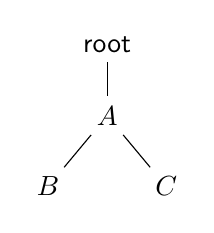
\begin{tikzpicture}
      \node {$\mathsf{root}$} [level distance=9mm] child {node {$A$} child {node {$B$}} child {node {$C$}}};
      \end{tikzpicture}
  };
  \node [rectangle,draw] (right) at (7,1.6) {
      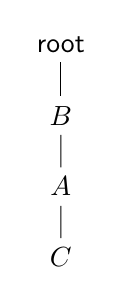
\begin{tikzpicture}
      \node {$\mathsf{root}$} [level distance=9mm] child {node {$B$} child {node {$A$} child {node {$C$}}}};
      \end{tikzpicture}
  };
  \node [rectangle,draw] (merge) at (4,-0.2) { ? };
  \node at (1.4,4.0) [text width=2.5cm,text centered] {Move $B$ to be a child of $A$};
  \node at (6.6,4.0) [text width=2.5cm,text centered] {Move $A$ to be a child of $B$};
  \draw [arrow] (start.west) -- (left);
  \draw [arrow] (start.east) -- (right);
  \draw [arrow] (left)  -- (merge.north west);
  \draw [arrow] (right) -- (merge.north east);
  \node at (4,0.6) {merge};
  %%%%%
  \node [rectangle,draw] at (9.9,4) {
      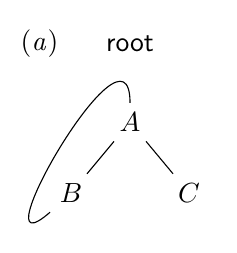
\begin{tikzpicture}
      \useasboundingbox (-1.3,-1.3) rectangle (1,1.2);
      \node at (-1.15,1.0) {(\emph{a})};
      \node at (0,1) {$\mathsf{root}$};
      \node (a1) {$A$} [level distance=9mm] child {node (b1) {$B$}} child {node {$C$}};
      \draw (b1.south west) .. controls (-2,-2) and (0,1.5) .. (a1.north);
      \end{tikzpicture}
  };
  \node [rectangle,draw] at (9.9,0.85) {
      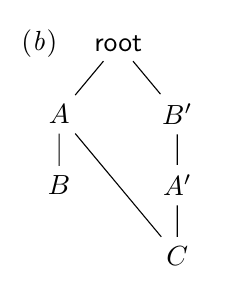
\begin{tikzpicture}
      \useasboundingbox (-1.15,-3.0) rectangle (1.15,0.2);
      \node at (-1.0,0.0) {(\emph{b})};
      \node {$\mathsf{root}$} [level distance=9mm] child {node (a2) {$A$} child {node {$B$}}} child {node {$B'$} child {node {$A'$} child {node (c2) {$C$}}}};
      \draw (a2) -- (c2);
      \end{tikzpicture}
  };
  \node [rectangle,draw] (start) at (12.5,4) {
      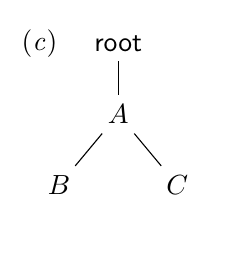
\begin{tikzpicture}
      \useasboundingbox (-1.15,-2.3) rectangle (1.15,0.2);
      \node at (-1.0,0.0) {(\emph{c})};
      \node {$\mathsf{root}$} [level distance=9mm] child {node {$A$} child {node {$B$}} child {node {$C$}}};
      \end{tikzpicture}
  };
  \node [rectangle,draw] (right) at (12.5,0.85) {
      \begin{tikzpicture}
      \useasboundingbox (-1.15,-3.0) rectangle (1.15,0.2);
      \node at (-1.0,0.0) {(\emph{d})};
      \node {$\mathsf{root}$} [level distance=9mm] child {node {$B$} child {node {$A$} child {node {$C$}}}};
      \end{tikzpicture}
  };
\end{tikzpicture}
\caption{Initially, $A$ and $B$ are siblings. $B$ is moved to be a child of $A$, while concurrently
$A$ is moved to be a child of $B$. Boxes (\emph{a}) to (\emph{d}) show possible outcomes of the merge.}\label{fig:concurrent-move}
\end{figure}

A more subtle kind of conflict is illustrated in Figure~\ref{fig:concurrent-move}.
Here, $B$ is moved to be a child of $A$, while concurrently $A$ is moved to be a child of $B$. 
If the CRDT does not take care to detect this situation, it may introduce a cycle in the merged result, as shown in Figure~\ref{fig:concurrent-move}(\emph{a});
this result is no longer a tree.
Handling such conflicting move operations is a challenging problem, and to our knowledge no existing implementation of a tree CRDT has found an adequate solution to this problem.

Several CRDT tree datatypes for XML \cite{Martin:2010ih,Nicolaescu:2015id} and JSON data \cite{Kleppmann:2016ve,Automerge,crjdt} have been developed, but to our knowledge, none of them define a move operation.
Tao et al.~\cite{Tao:2015gd} implemented a CRDT-based replicated filesystem, resolving concurrent moves with an approach illustrated in Figure~\ref{fig:concurrent-move}(\emph{b}): conflicting branch nodes (directories) are duplicated, and leaf nodes (files) may be referenced from multiple branch nodes.
Thus, Tao et al.'s data structure is strictly a DAG, not a tree.

Najafzadeh~\cite{Najafzadeh:2017vk,Najafzadeh:2018bw} also implemented a CRDT-based replicated filesystem, but chose a different approach: move operations must acquire a global lock before they can proceed, which ensures that conflicting concurrent move operations cannot occur in the first place.
This conservative approach rules out move conflicts, but the resulting datatype is not strictly a CRDT, since some operations require strongly consistent synchronisation.


\subsection{Specifying a Tree with Atomic Moves}\label{sec:tree-spec}

We now demonstrate the power of the OpSets approach by using it to define a tree CRDT with an anomaly-free atomic move operation.
Our specification rules out violations of the tree structure such as those in Figure~\ref{fig:concurrent-move}(\emph{a,b}), and concurrent moves do not duplicate tree nodes.
Moreover, our CRDT does not require any locks or global synchronisation.

When the OpSet contains conflicting move operations, our specification chooses one of them as the one that takes effect, and simply ignores the other conflicting operations.
Thus, in the example of Figure~\ref{fig:concurrent-move}, the merged outcome of the two conflicting move operations is either (\emph{c}) or (\emph{d}).
If two users concurrently move the same item to different locations, the move operation with the greater ID determines the item's final location.
However, in non-conflict situations, all concurrent move operations take effect.

We define a tree to be a restricted form of the object graph specified in \S~\ref{sec:datatypes}.
First, we require that there is a designated root object: assume that we have an operation ID $\mathsf{root}$ that is less than all other operation IDs (according to the total order on identifiers, introduced in \S~\ref{sec:system-model}).
Further assume that for any OpSet $O$ specifying a tree, we have either $(\mathsf{root},\, \mathsf{MakeList}) \in O$ or $(\mathsf{root},\, \mathsf{MakeMap}) \in O$, depending on whether the root node is a list or a map.
We define an object $x$ to be the \emph{parent} of an object $y$ if one of the values in $x$ is a reference to $y$.
The \emph{ancestor} relation is the transitive closure of the parent relation, defined using the element relation $E$:
\begin{align*}
    \mathsf{parent}(E,\, i) &=
    \begin{cases}
        \big\{ (\mathit{obj}, \mathit{val}) \mid \exists\,\mathit{id}, \mathit{key}.\;
            (\mathit{id}, \mathit{obj}, \mathit{key}, \mathit{val}) \in E \big\} & \text{if } i=1 \\
        \big\{ (x, z) \mid (x, y) \in \mathsf{parent}(E,\, i-1) \;\wedge\;
            (y, z) \in \mathsf{parent}(E,\, 1) \big\} & \text{if } i > 1
    \end{cases} \\[8pt]
    \mathsf{ancestor}(E) &= \bigcup_{i \;\geq\; 1} \mathsf{parent}(E,\, i)
\end{align*}

An object graph is a tree if the root has no parent, every non-root node has exactly one parent, and if the ancestor relation has no cycles.
We can redefine the operation interpretations from \S~\ref{sec:datatypes-interp} to preserve this tree invariant.
In fact, it is sufficient to redefine only the interpretation of $\mathsf{Assign}$, and to leave the interpretation of the other five operation types unchanged:
\begin{align*}
    \mathsf{interp}&\big[(E,\, L),\; (\mathit{id},\, \mathsf{Assign}(\mathit{obj}, \mathit{key}, \mathit{val}, \mathit{prev})) \big] \;=\\
    & \left\{
    \arraycolsep=0pt \def\arraystretch{1.5}
    \begin{array}{l}
        (E,\, L) \qquad \text{if } (\mathit{val},\, \mathit{obj}) \in \mathsf{ancestor}(E) \\[2pt]
        \Big( \big\{ (\mathit{id}', \mathit{obj}', \mathit{key}', \mathit{val}') \in E \mid
        \mathit{id}' \notin \mathit{prev} \wedge \mathit{val}' \neq \mathit{val} \big\} \;\cup\;
        \big\{ (\mathit{id}, \mathit{obj}, \mathit{key}, \mathit{val}) \big\},\; L \Big) \\
        \hphantom{(E,\, L)} \qquad \text{if } (\mathit{val},\, \mathit{obj}) \notin \mathsf{ancestor}(E)
    \end{array} \right.
\end{align*}

This definition differs in two ways from that in \S~\ref{sec:datatypes-interp}.
Firstly, the operation has no effect if $\mathit{val}$ is already an ancestor of the proposed parent $\mathit{obj}$, since the operation would otherwise introduce a cycle.
Secondly, any existing tuple in $E$ that references the same value $\mathit{val}$ is removed, preserving the invariant that every non-root node must have exactly one parent.

This interpretation of $\mathsf{Assign}$ performs an atomic move whenever $\mathit{val}$ is the ID of an existing object in the tree; in that case, it is moved from its existing position to the key $\mathit{key}$ in the object $\mathit{obj}$.
If $\mathit{val}$ does not currently exist in the tree (e.g.\ because it has just been created), the operation behaves like conventional assignment.

\section{Related Work}\label{sec:relwork}

\subsection{Interpretation of Operation Sequences}\label{sec:op-sequences}

The general idea of establishing a total order of operations, and executing them in that order, appears in many areas of computing:
for example, in the state machine approach to replication \cite{Schneider:1990vy},
the event sourcing approach to data modelling \cite{Vernon:2013ww},
write-ahead logs for crash recovery \cite{Mohan:1992fe},
serializable transactions \cite{Davidson:1985hv},
and scalable multicore data structures \cite{BoydWickizer:2014uz}.
However, beneath the superficial similarity of these approaches there are important differences that need to be distinguished.

As discussed in \S~\ref{sec:order-change}, many of these systems rely on the property that after some operation is executed, all subsequent operations will appear \emph{after} it in the total order.
In other words, the operation sequence is an append-only log, and new operations never need to be inserted ahead of an existing operation in the total order.
This is a very strong property: in the context of a distributed system, it requires an atomic broadcast (or total order broadcast) protocol \cite{Defago:2004ji}, which is equivalent to solving distributed consensus \cite{Chandra:1996cp}.
This class of protocols requires communication with a quorum of nodes in order to make progress \cite{Howard:2016tz}, and it cannot guarantee progress in a fully asynchronous setting \cite{Fischer:1985tt}.

By contrast, the sequential OpSet interpretation of \S~\ref{sec:op-serial} does not require atomic broadcast because it allows operations to be added to the OpSet in any order, and it assigns operation IDs without any coordination.
Few systems use this approach; the most closely related prior work are the Bayou system \cite{Terry:1995dn}, which executes tentative transactions deterministically in timestamp order, and Burckhardt's \emph{standard conflict resolution} \cite[\S~4.3.3]{Burckhardt:2014hy}.
Both of these share the OpSet approach's characteristic that operations with a higher ID need to be undone and re-applied when a new operation with a lower ID is received.

Our contribution in this paper is to formulate the OpSet approach more generally as a tool for specifying and reasoning about complex replicated data structures, such as lists and trees.
Our work is the first to use this approach in mechanised proofs, in which we show that a non-OpSet list CRDT (RGA) satisfies an OpSet-based specification, and prove the absence of the interleaving anomaly in Figure~\ref{fig:bad-merge}.

Baquero et al.~\cite{Baquero:2014ed} and Grishchenko~\cite{Grishchenko:2014eh} have proposed representing CRDTs in terms of a partially-ordered log of operations, where the partial order captures the causal relationships between operations.
The OpSet approach can be seen as a variant of this idea, in which we define the total order on identifiers to be a linear extension of the partial order.

\subsection{Specification and Verification of Replicated Datatypes}

Algorithms for collaboratively editing a shared data structure have been the topic of active research for approximately 30 years, under the headings of Operational Transformation \cite{Ellis:1989ue,Ressel:1996wx,Sun:1998vf,Oster:2006tr} and CRDTs \cite{Shapiro:2011wy,Shapiro:2011un}.
However, throughout this time, the exact consistency properties provided by the algorithms have been somewhat unclear.
For example, Sun et al.~\cite{Sun:1998un} identified three desirable properties that they articulated informally: \emph{convergence}, \emph{causality preservation}, and \emph{intention preservation}.
While the definition of the first two properties is fairly unambiguous, the definition of ``intention preservation'' leaves much more room for interpretation.
Efforts to formally specify and verify the semantics of replicated datatypes have replaced such informal statements with precise consistency properties.

Burckhardt et al.~\cite{Burckhardt:2014ft} provide a wide-ranging formal account of CRDTs, covering their specification, verification, and optimality, with the semantics of an operation on a replicated datatype given as a function of the operation, $o$, and a \emph{operation context}---the set of operations visible to a node at the time that $o$ was received.
Our OpSets can be seen as an explicitly executable variation on this idea: nodes record all operations that they have ever received in a monotonically growing set, and the interpretation function builds the result ``bottom up'' in a fold-like operation.
In contrast to Burckhardt et al., who focus on applying their techniques to set and counter datatypes, we apply our approach to the specification of lists, maps, and trees, using our OpSets as a tool for designing new replicated datatypes---including those previously thought impossible, such as our replicated tree with atomic move.
Gotsman et al.~\cite{DBLP:conf/popl/GotsmanYFNS16} extend Burckhardt et al.'s formalism to reason about hybrid consistency models, providing a modular proof rule inspired by permissions-based logics to enforce an integrity invariant for a given consistency model.

Bieniusa et al.~\cite{Bieniusa:2012gt} articulate a \emph{principle of permutation equivalence} that partially specifies the expected semantics of replicated datatypes, but which leaves some combinations of operations unspecified.
Zeller et al.~\cite{Zeller:2014fl} formalise counters, registers, and sets using Isabelle/HOL and provide mechanised proofs of their correctness.
Attiya et al.~\cite{Attiya:2016kh} give two specifications of collaborative text editing ($\mathcal{A}_\textsf{strong}$ and $\mathcal{A}_\textsf{weak}$), prove that the RGA CRDT \cite{Roh:2011dw} satisfies $\mathcal{A}_\textsf{strong}$, and conjecture that the Operational Transformation algorithm Jupiter \cite{Nichols:1995fd} satisfies $\mathcal{A}_\textsf{weak}$.
Wei et al.~\cite{Wei:2017tg} complete the proof that Jupiter satisfies $\mathcal{A}_\textsf{weak}$.

In our prior work \cite{Gomes:2017gy} we establish a formal verification framework for CRDTs in Isabelle/HOL, and verify the strong eventual consistency properties (in particular, convergence) of a list, set, and counter datatype.
The Isabelle implementation of RGA we use in \S~\ref{sec:datatypes} is based on this work \cite{Gomes:2017vo}.
However, this work does not specify the datatype semantics beyond the convergence property.

Gaducci et al.~\cite{DBLP:conf/coordination/GadducciMR17} develop a semantics for replicated datatypes, placing a focus on compositionality, where a replicated datatype is modelled as a function from labelled directed acyclic graphs of events to sets of values, with each value in this set potentially observable at a node under different ordering of events observed at that node.
A notion of behavioural \emph{refinement} for replicated datatypes induced by set inclusion is also defined, along with a generalisation of their relational semantics to a categorical one.

Mukund et al.~\cite{DBLP:conf/atva/MukundRS15} use traces to provide bounded declarative specifications of CRDTs and show how Counter Example Guided Abstract Refinement (CEGAR) can be used to automatically verify a reference CRDT implementation against its bounded specification.

\subsection{Collaborative Tree Datatypes}

For collaborative editing of tree data structures, several CRDTs \cite{Martin:2010ih,Kleppmann:2016ve} and Operational Transformation algorithms \cite{Jungnickel:2016cb,Ignat:2003jy,Davis:2002iv} have been proposed.
However, most of them only consider insertion and deletion of tree nodes, but do not support a move operation.

As explained in \S~\ref{sec:tree}, supporting an operation that can move a subtree to a new location within a tree introduces new conflicts that need to be handled.
Ahmed-Nacer et al.~\cite{AhmedNacer:2012us} survey approaches to handling these conflicts without providing concrete algorithms.
Tao et al.~\cite{Tao:2015gd} propose handling conflicting move operations by allowing the same object to appear in more than one location; thus, their datatype is strictly a DAG, not a tree.

Najafzadeh~\cite{Najafzadeh:2017vk,Najafzadeh:2018bw} asserts that concurrent move operations on a tree cannot safely be implemented in a CRDT, since the precondition of a move operation is not stable.
Najafzadeh suggests the use of locks to globally synchronise move operations, preventing a scenario such as that in Figure~\ref{fig:concurrent-move} from ever occurring.
However, the resulting datatype is not strictly a CRDT, since some operations require strongly consistent synchronisation.

To our knowledge, our move semantics specified in \S~\ref{sec:tree} is the first definition of such an operation on a fully asynchronous tree CRDT.
We avoid the apparent contradiction with Najafzadeh's assertion by evaluating the precondition $(\mathit{val},\, \mathit{obj}) \notin \mathsf{ancestor}(E)$ at the same time as applying the operation, rather than at the time when the operation is generated, and by applying all operations in the OpSet in a deterministic order.


\section{Conclusion}

TODO

\bibliographystyle{plainnat}
\bibliography{references}{}
\end{document}
